\documentclass[12pt]{article}
\usepackage[english]{babel}
\usepackage[utf8x]{inputenc}
\usepackage[T1]{fontenc}
\usepackage{lab}
\usepackage{listings}


\Instructors{Alex Mussa, Kevin Johnson}
\LabNumber{3}
\LabTitle{Circuit Prototyping and Testing}
\LabDate{July 1st, 2019}

\lstset{style=mystyle}

\begin{document}
\MakeLabPrelimTop

\section{Potentiometers}

Potentiometers are very important in circuits as they can vary the resistance seen between some contact points on the potentiometer such that the voltage in the center terminal varies proportionally with the variation of resistance. In such a way, potentiometers are great for performing tasks such as controlling the volume of an audio signal and adjusting the brightness of a light such as in a sliding light switch. The potentiometer shown in \textit{Figure 1} below is an example of a potentiometer designed for use in circuit prototyping with a breadboard.

\begin{figure}[H]
\begin{subfigure}{.5\textwidth}
    \centering
    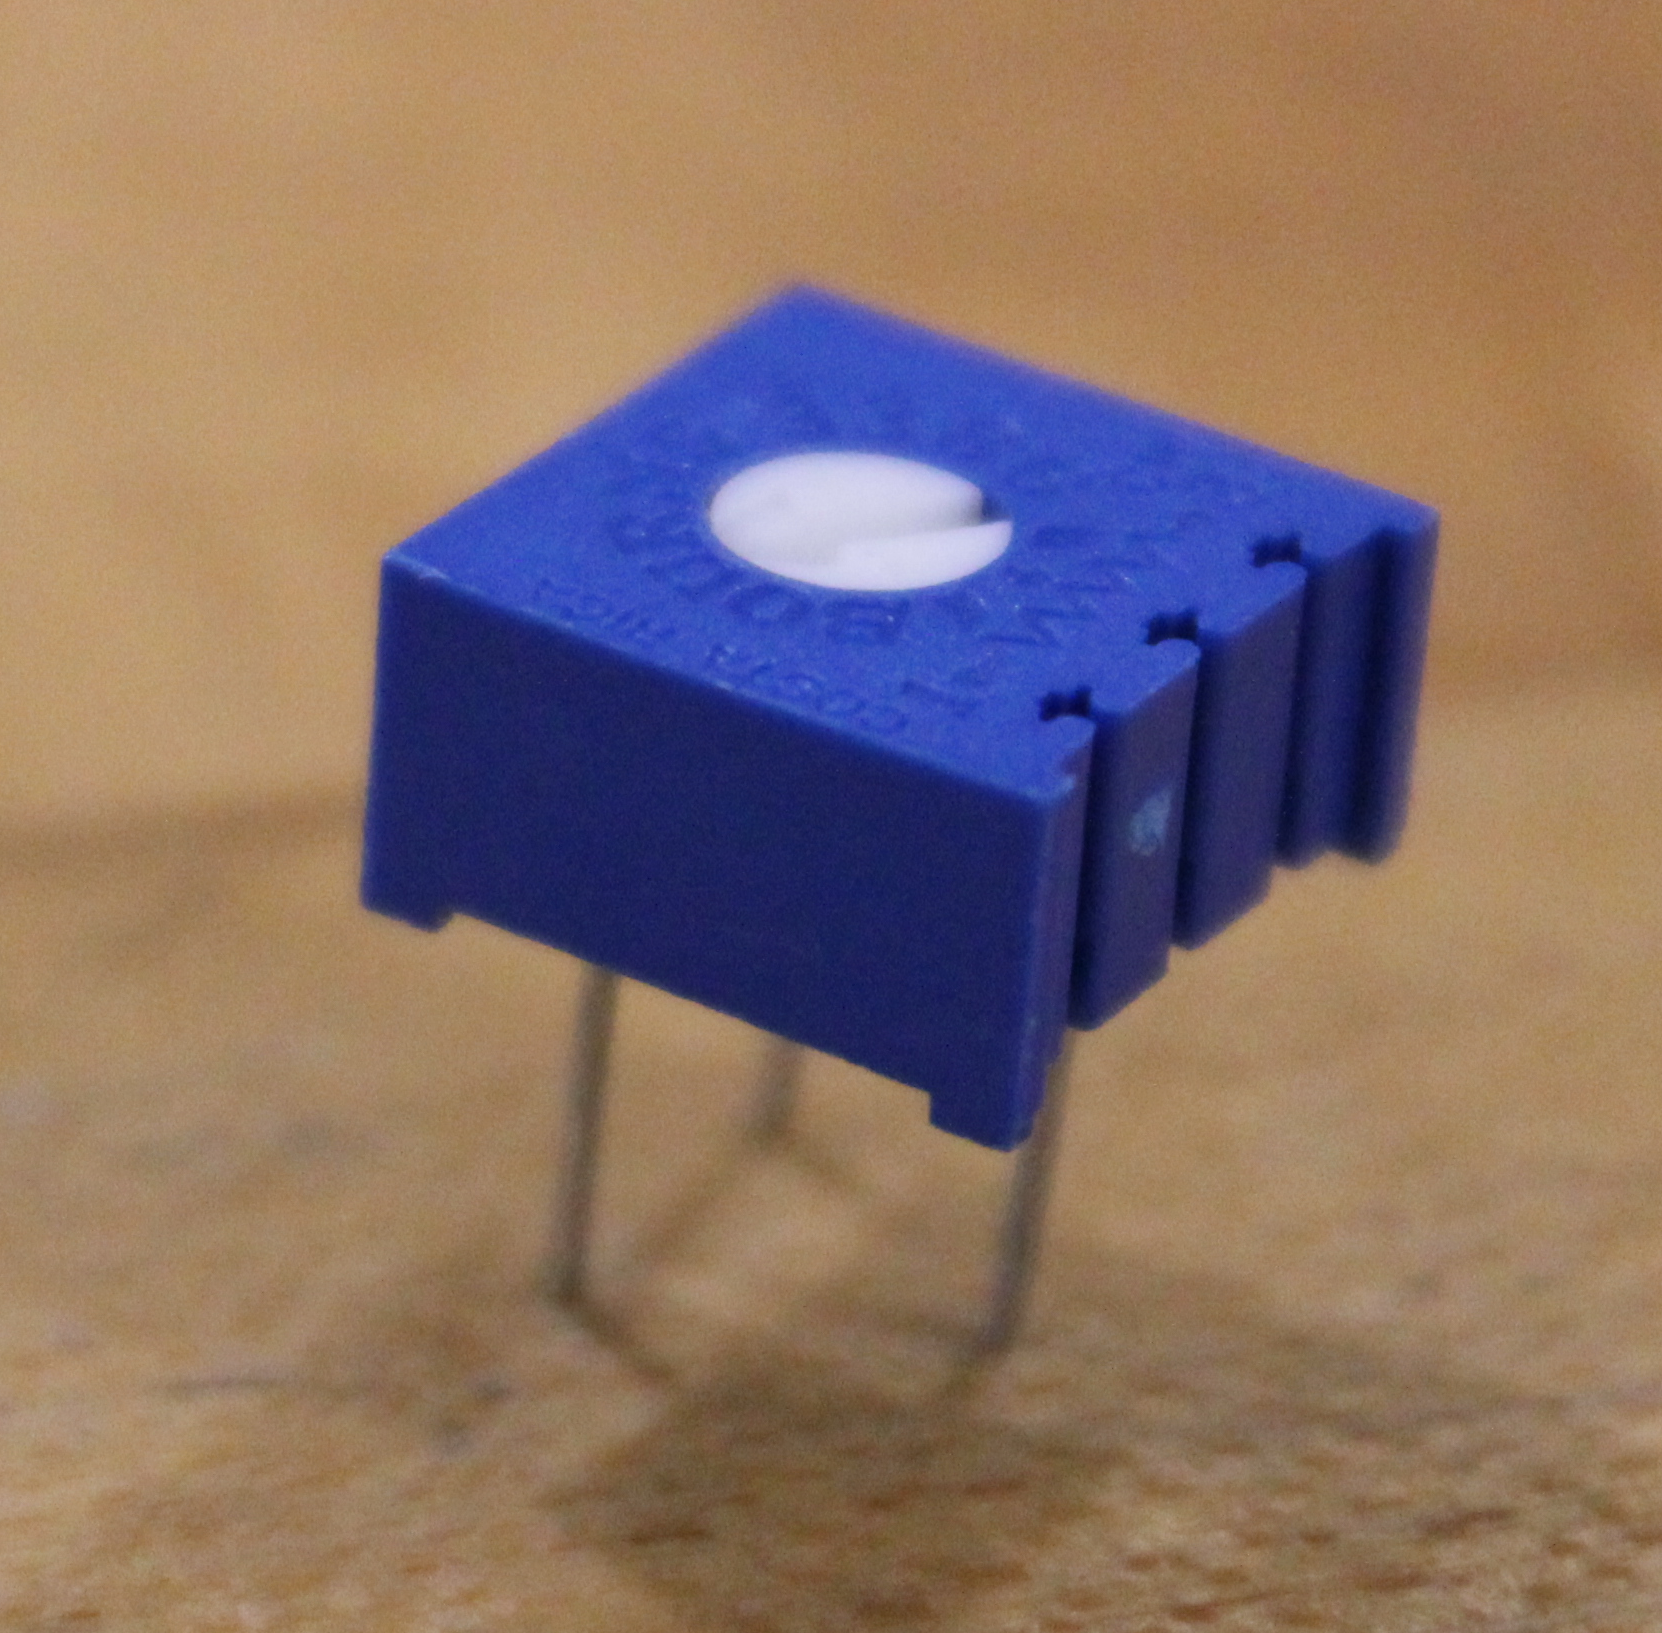
\includegraphics[width=0.8\linewidth]{photos/prelim/pot.png}
    \caption{Top view.}
\end{subfigure}%
\begin{subfigure}{.5\textwidth}
  \centering
  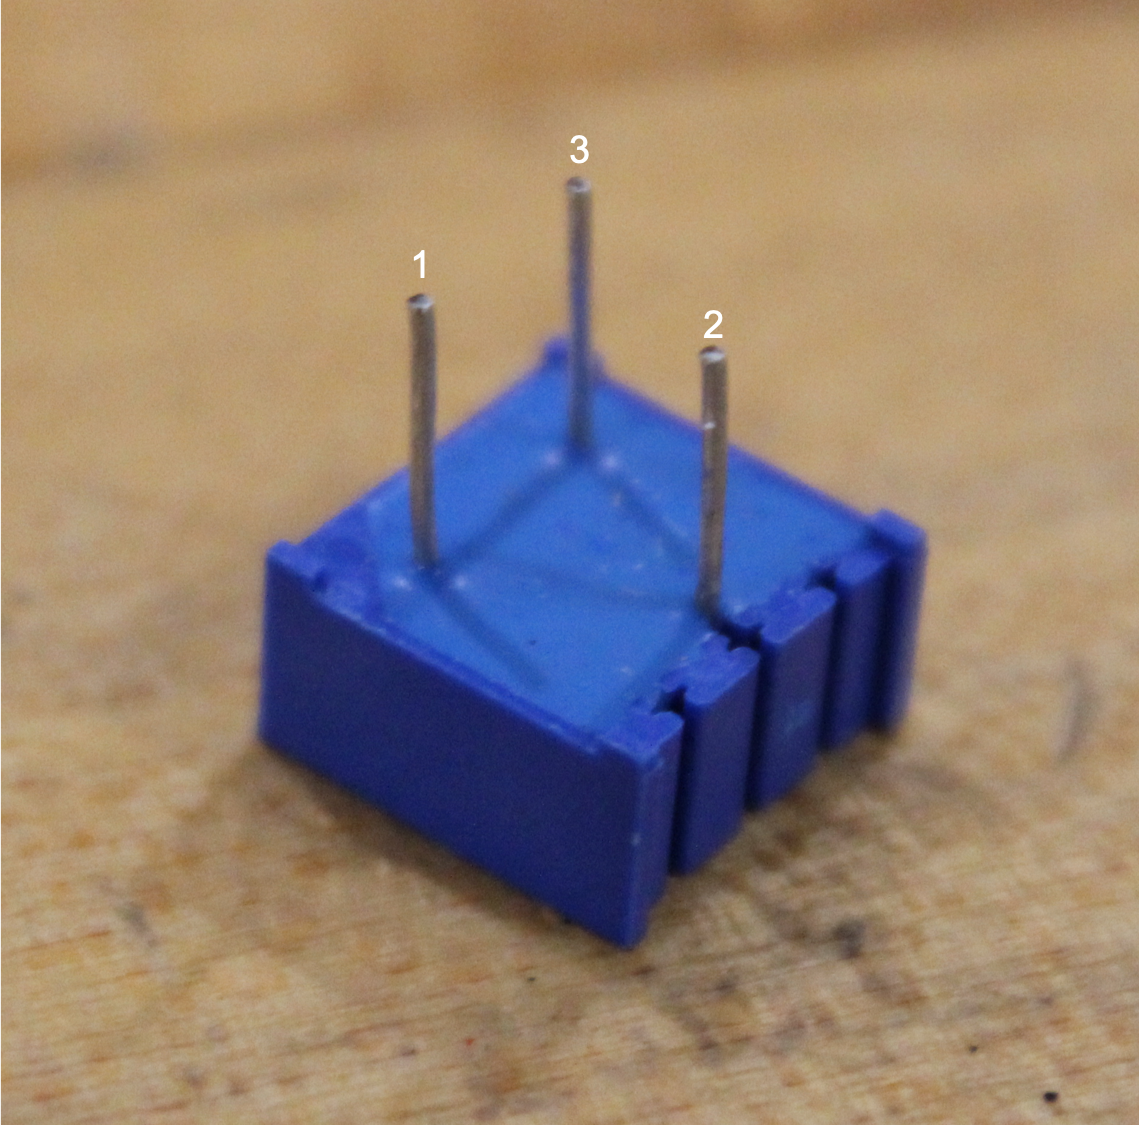
\includegraphics[width=0.79\linewidth]{photos/prelim/potlabeled.png}
  \caption{Bottom view.}
\end{subfigure}
\caption{Top and bottom view of a potentiometer.}
\end{figure}

The potentiometer, referred to as a pot, is in essence a resistor that has a "tap" connection in the middle. In this sense, the potentiometer can be thought of as two resistors in series that together add up the the rating of the potentiometer, but whose resistances can be altered with a knob. Consider the equivalent circuit schematic for a potentiometer in \textit{Figure 2} below. In this figure, the two resistors represent the resistances between terminals 1 and 2 in the case of the top resistor, R1 and between terminals 2 and 3 in the case of the bottom resistor, R2. 

\begin{figure}[H]
    \centering
    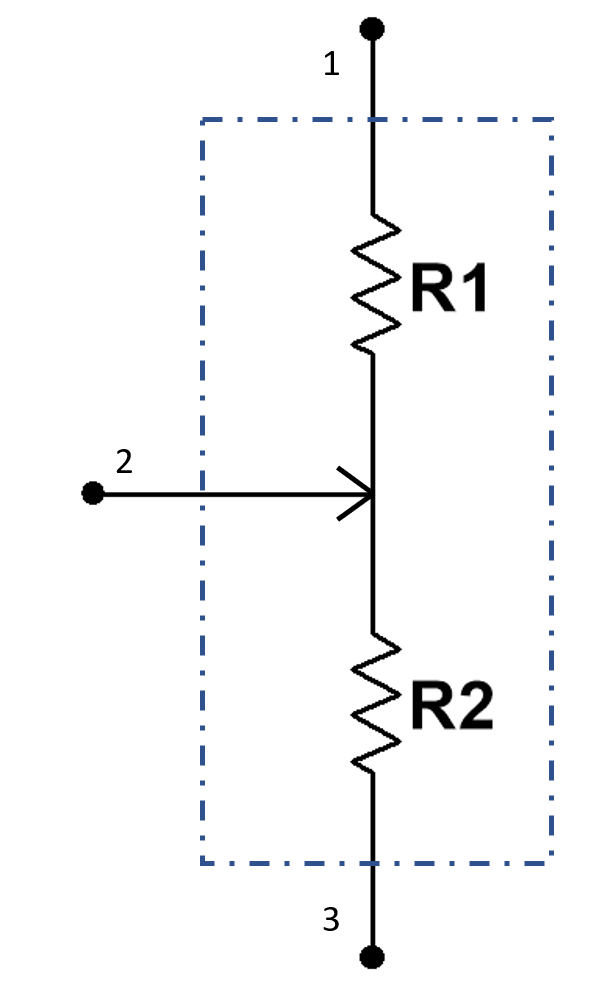
\includegraphics[width=6cm]{photos/prelim/potschem.PNG}
    \caption{An equivalent circuit schematic of the internal workings of a potentiometer.}
\end{figure}

The potentiometer works such that when you turn the white knob on the top of the potentiometer, the \textit{wiper} connected to pin 2 moves and adjusts the resistor values of R1 and R2. It is such that the series resistance of R1 and R2 always remain the rating of the potentiometer. For example, consider a $10k\Omega$ potentiometer. When the potentiometer is turned $0\%$ of the way from pin 1 to pin 3, that means that R1 is approximately $0\Omega$ and all of the resistance of the potentiometer is between pin 2 and pin 3. As the wiper at pin 2 is turned towards pin 3, R1 increases as R2 decreases. As such, the resistances between the pins for different percentages of turning the wiper of pin 2 away from pin 1 for any potentiometer with resistance R would be as follows:

\begin{table}[H]
    \centering
    \begin{tabular}{|c||l|l|}
        \hline
        \% turn of wiper from pin 1 & R1 & R2  \\ \hline \hline
        $0\%$                       & $0*R$   & $1*R$     \\ \hline
        $25\%$                      & $0.25*R$   & $0.75*R$     \\ \hline
        $50\%$                      & $0.5*R$   & $0.5*R$     \\ \hline
        $75\%$                      & $0.75*R$  & $0.25*R$     \\ \hline
        $100\%$                     & $1*R$   & $0*R$     \\ \hline
    \end{tabular}
    \caption{}
\end{table}

Intuitively, you can interpret this table as showing that when the wiper at pin 2 is turned 100\% of the way towards pin 3, all of the resistance lies between pin 1 and 2 and none of the resistance between 1 and 2. This is because the wiper is now at pin 3 and as such is "connected" internally to pin 3, meaning the only material between pin 2 and 3 is primarily conductive materials. Since the potentiometer has some R value of resistance between pins 1 and 3 internally, all of this resistance is seen between pins 1 and 2.

Consider that the voltage applied between pins 1 and 3 is 5V, such as that seen in \textit{Figure 3}, for the following example.

\begin{figure}[H]
    \centering
    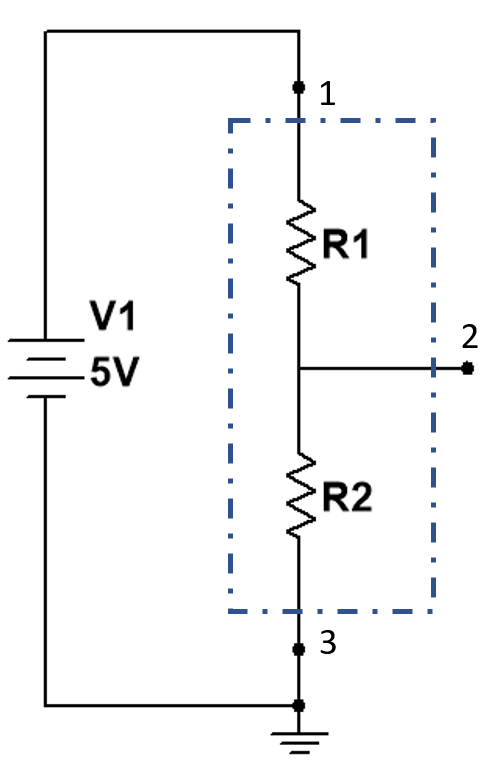
\includegraphics[width=6cm]{photos/prelim/voltagedivider.PNG}
    \caption{An potentiometer with voltage applied across pins 1 and 3.}
\end{figure}

in this figure, the voltage would be "divided" between the two resistors, where the more significant voltage will be dropped across the larger resistor, as dicated by the equivalent resistance being $R = R_{1} + R_{2}$. The current flowing from the power supply can be calculated $I = \frac{V_{1}}{R}$ and each resistors voltage drop as $V_{R1} = I * R_{1}$ and $V_{R2} = I * R_{2}$. Thus, varying the resistance ratio between R1 and R2 such as done with the knob on the potentiometer, will change $V_{R2} = \frac{5V * R_{2}}{R_{1}+R_{2}}$ which is the voltage between pins 2 and 3.

The importance of this is the ability for a user to interface with the circuit and set the voltage at some point. This can be for interfacing with the microcontroller to tell it the speed to perform some task at, for example or alter some other parameter of a circuit. Another example is that this can be input into a microcontroller to tell it how to operate. Understanding a potentiometers internal operation is important to understanding how to utilize it in such applications in a design.

\section{Switches}

Another common circuit element used to control the delivery of a voltage to a device is a switch. A switch can enable or disable any portion of a circuit that comes after the switch, as it is designed to internally break the conductive material and allow no current to flow. In this respect, potentiometers can vary the amount of a signal supplied to a given part of a circuit, where a switch either permits or denys the signals completely.

There are many different type of switch, from very simple switches such as the ones found in pushbuttons and lighting applications, to ones that require tapping, thermal energy, or light to activate. These different types of switches can be used for different applications, varying from simply enabling or disabling power to a device to detecting a severe rise in temperature or the presence of light. In this lab, we will explore the basic pushbutton found in the 37 sensors kit as seen below.

\begin{figure}[H]
    \centering
    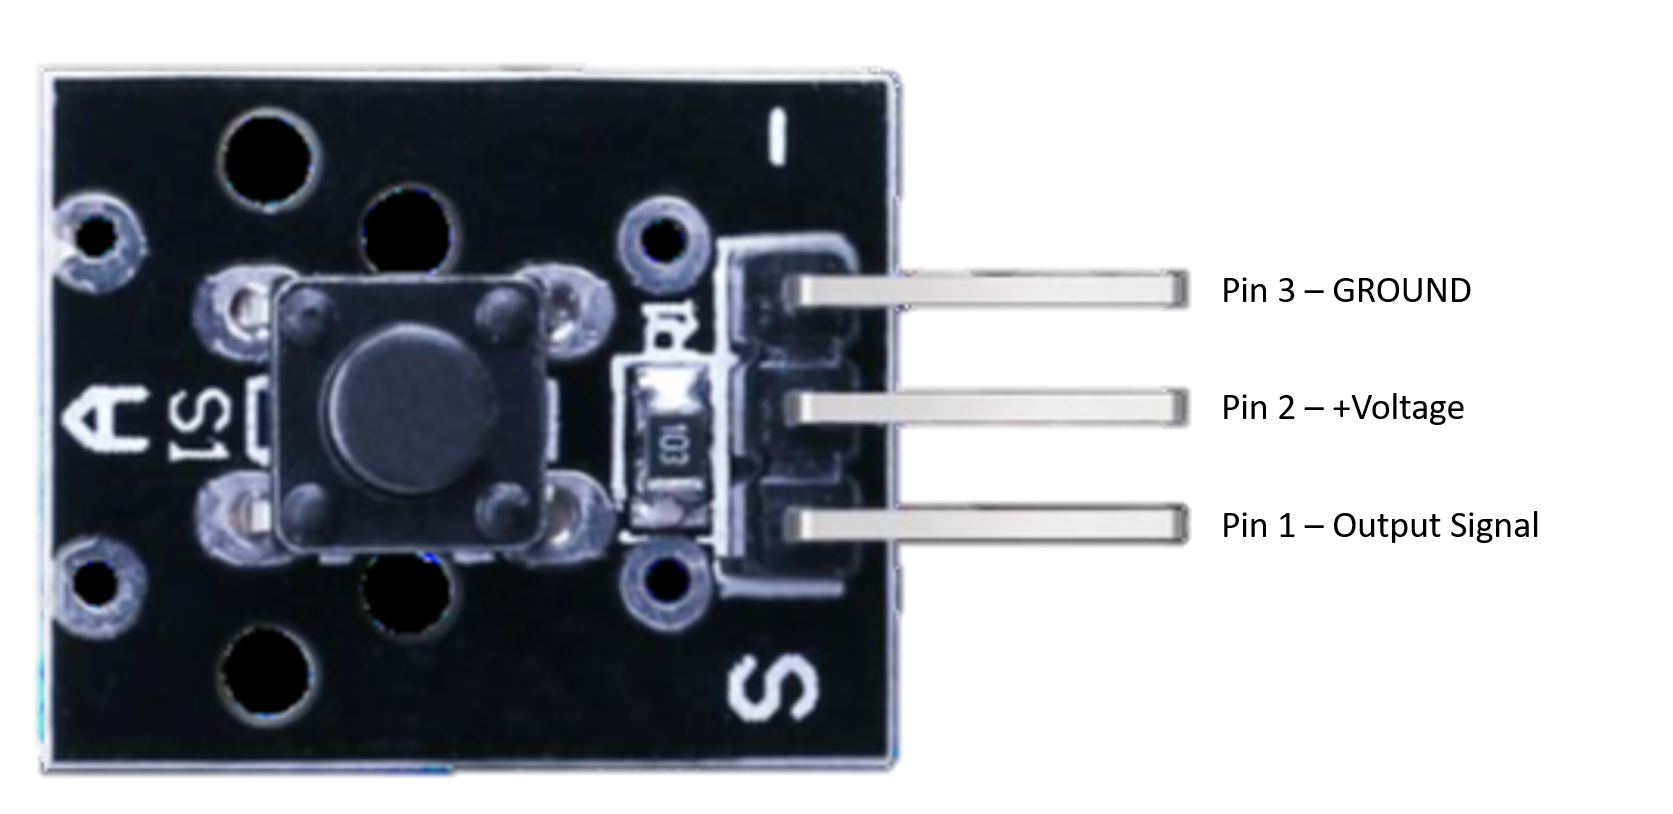
\includegraphics[width=12cm]{photos/prelim/pushbutton.PNG}
    \caption{A pushbutton found in the 37 sensors kit.}
\end{figure}

For the switch, the +5V signal is either passed or denied, based on if the pushbutton is pressed or not. If the pushbutton is pressed, the voltage seen at the output when compared to ground will be the same as the voltage applied at Pin 2 and current will be able to flow to any circuit elements connected. Otherwise, the connection between the input and output will be broken.

Some applications of this include some simple press to activate device, such as a flashlight that requires you to hold the button. When you press the button, current can flow to the bulb and illuminate it where if you release, it will turn off. Also, the end device receiving the output signal could be a microcontroller who can do a lot with this signal. For example, this could simply control the power supplied to an LED connected to the arduino or can be used for more advanced applications such as selecting a mode for the self-balancing robot to be in. In this application, the microcontroller could count the amount of times the button has been pressed and put it into various modes, such as self-following and glow mode.

\section{Controlling circuits with Alternating Current Waveforms}

Some circuit element behaviors can be "controlled" based on the voltage that is supplied to it. For example, the brightness of an LED can be varied based on the voltage that is applied to it. As such, an alternating voltage waveform can be utilized to control some circuit element, such as motors and LEDs.

\subsection{Sine Waves}

A commonly used waveform for AC signals is the sine wave. The thing to note about the sine wave is the voltage values vary in a non-linear manner except at the discrete points of when the amplitude is zero. The sine wave has continuously changing amplitudes, such that within an interval of time T, the change in amplitude maybe be small or large. In this sense, the amount of change occurring in some small interval of time may be more or less than in the next interval. This can be exemplified through \textit{Figure 5}.

\begin{figure}[H]
    \centering
    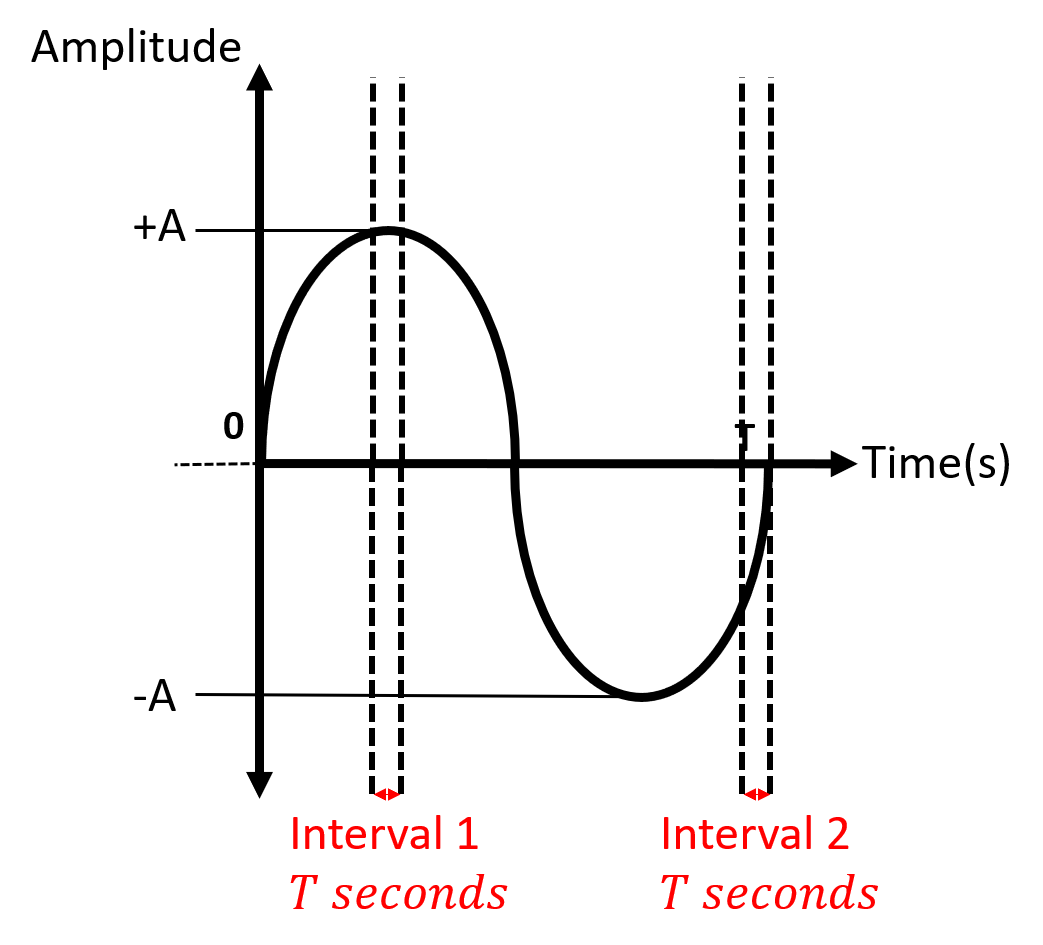
\includegraphics[width=12cm]{photos/prelim/sine.png}
    \caption{An example of different alternating conditions in a sine wave.}
\end{figure}

In interval 1, the sine waves amplitude doesnt change much. This si due to the fact the sine wave is transitioning back to the negative part of the signal and the amplitude remains primarily flat. In interval 2, the sine wave is in one of its steepest transition areas and the amplitude varies much quicker. 

\subsection{Triangle Waves}
 The triangle wave shares most of its parameters with the sine wave, but difers from the sine wave because it is said to be "peicewise linear". What this means is that the triangle wave is linear in "pieces". Take for example the region between the highest peak and lowest peak shown in \textit{Figure 6}. 

\begin{figure}[H]
    \centering
    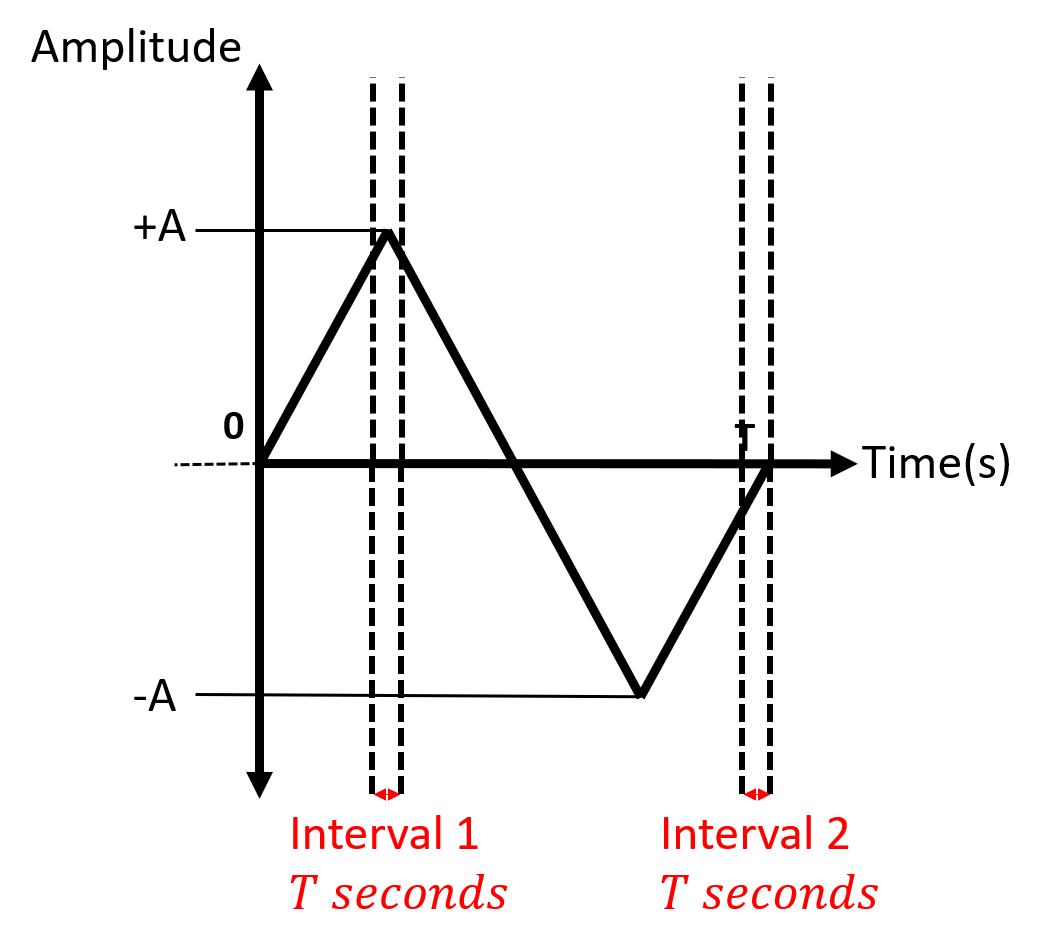
\includegraphics[width=12cm]{photos/prelim/triangle.png}
    \caption{An example of the discontinuous and continuous alternating conditions in a triangular wave.}
\end{figure}

If you neglect the rest of the graph to the left of the highest peak shown in interval 1 and right of the lowest peak, the plot look like a linear function, such as the one the could take the form $y = mx + b$ where $m$ is slope and $b$ is y intercept. This mean it has a constant slope within this region and it does not change. The triangular wave is not only piecewise linear in this region, but also within the region that transitions from the negative peak to positive shown by interval 2. Any interval of time T that stay within the peaks will have the same slope. 

\subsection{Square Waves}

A square wave can be intuitively related to turning on and off a DC voltage at a constant rate every second. This can be observed in the waveform in \textit{Figure 7} However, the square wave has some additional parameters that specify its shape and behavior. The square wave has the parameters of frequency and peak to peak voltage but also need further specification of offset and an unique parameter duty cycle.

\begin{figure}[H]
    \centering
    
\includegraphics[width=12cm]{photos/prelim/square.png}
    \caption{A square wave.}
\end{figure}

In the figure, the peak voltage of the waveform is $\frac{A}{2}$, the peak to peak is $V_{pp} = A$, and the frequency is $f = \frac{1}{T}$. However, notice that the waveform does not vary from an amplitude of $+\frac{A}{2}$ to $-\frac{A}{2}$, but from A to 0. This is because the square wave has been "offset" in amplitude by $+\frac{A}{2}$. This means that every values the square wave takes has $+\frac{A}{2}$ added to it, causing the shift upwards in the graph. This offset can be done to any AC signal.

The square wave, however, also has a specification of duty cycle. this value specifies the percentage of one period of the signal that the waveform is positive. In the figure, the waveform has a duty cycle of 50\% , as half of the period is positive and half is negative. For higher percentage duty cycles, the period contains a longer duration of the positive amplitude.

Square waves are great for saving power, as instead of supplying current for the full duration of an interval of time, it can be turned on and off. DC mototrs and LEDs, for example, can benfit from this. In LEDs, as the human eye can only process images at a certain rate, an LED can flash at a certain frequency with a certain on duration and effectively save power and be unnoticeable to the viewer. 

LEDs and other devices can save power over the use of DC in that within some period of time T, the square wave has a lower average voltage supply. Considering \textit{Figure 7} as a voltage waveform where amplitude represents volts, the voltage is not continuously supplied in the duration of the period T like a DC signal would. Instead, it alters from generating potentially to not rapidly. As such, within a period of a square wave an average amount of voltage can be computed from the duty cycle. If the duty cycle of the square wave is 25\%, for example, the average amount of volts supplied during a single period T seconds of the waveform would be the duty cycle times the amplitude, $V_{avg} = A * \frac{1}{4} = \frac{A}{4}$. By supplying less voltage in a single period of time, the amount of power is reduced.

\subsection{Pulse Width Modulation}

By changing the width of the "pulse" in the square wave, square waves can be used to do things such as vary motor speed. For example, consider a 25\% duty cycle square wave with offset as shown in \textit{Figure 6}. In any given period, the average voltage would be exactly $V = 0.25 * A = \frac{A}{4}$. In this sense, increasing the duty cycle will increase the voltage supplied. This variation of the width of the pulse of a square wave is the essence of pulse width modulation and can be utilized for varying the speed a DC motor spins in a robots controls, for example.

By supplying different average voltages, the motor will spin slower or faster. Higher average voltages found in higher pulse widths will cause it to spin faster. Lower average voltages will cause it to spin slower as less power is being consumed by the motor. Thus, "modulating" or changing rapidly the widths of the pulse can allow a microcontroller to control the motion of a robot through the control of the spin of a motor.

\section{DC Motor Control}

Electric motors are very useful electrical devices found in a wide array of applications such as vehicles, children's toys, heavy machinery, manufacturing facilities, robotics, etc. The ability of a motor to convert electrical energy into mechanical energy enable these devices to perform such tasks. Specifically for robotics controls, DC motors are typically utilized for their abilities to easily interface with microcontrollers for motion control with the use of PWM. 

As DC motors can easily be turn on by applying a DC voltage and off by removing the voltage, the waveform seen in \textit{Figure 7} would be able to achieve this. When the signal is at +A, the motor will be on and when its at 0, it will be off. In this sense, all that need to be done is power needs to be either fed to the motor at some times and not fed. This could be accomplished by turning a switch on and off very quickly for example. Although a microntroller cannot provide the power needed to control a robot, it can control a fast-acting "switch" that would turn on and off power to the motor. In this sense, a microcontroller can easily interface with the motors to control its speed and direction.

In the Tumbller self-balancing robot, the arduino microntroller sends a few signals to indicate operating mode such as direction of travel as well as the PWM signal to a chip called the Toshiba TB6612FNG. This chip inputs power and these signals and performs the task of appropriately supplying the power to the motors to control the right direction and magnitude of the spin of two DC motors. The pins control code from the datasheet can be seen below in \textit{Figure 8}.

\begin{figure}[H]
    \centering
    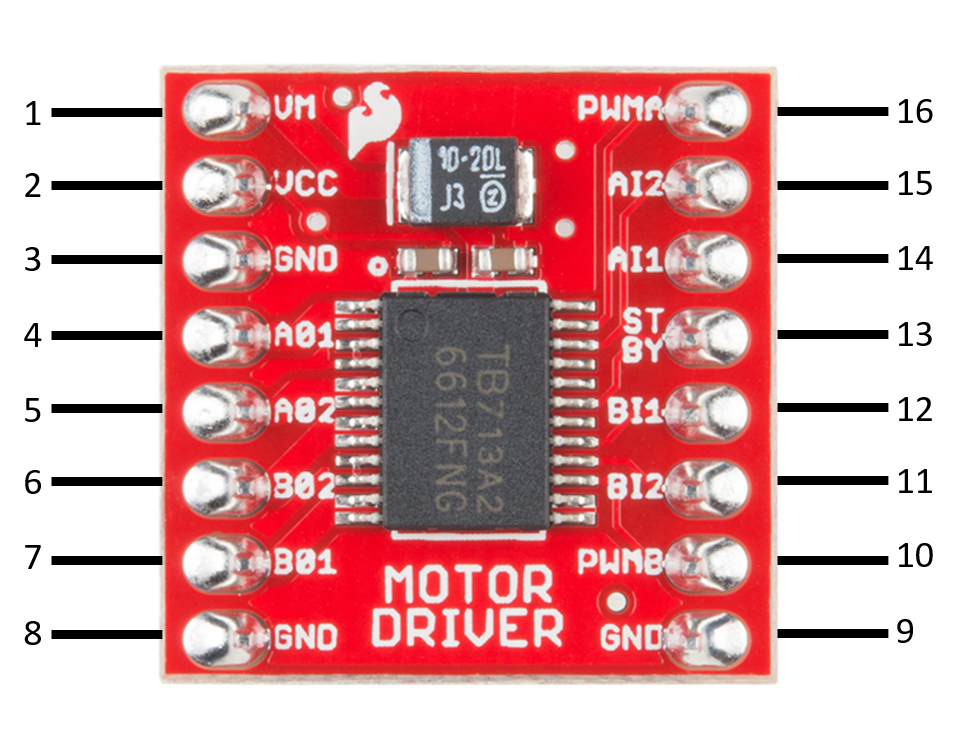
\includegraphics[width=12cm]{photos/lab/motordriver.png}
    \caption{The Toshiba TB6612FNG's pinout diagram.}
\end{figure}

\begin{figure}[H]
    \centering
    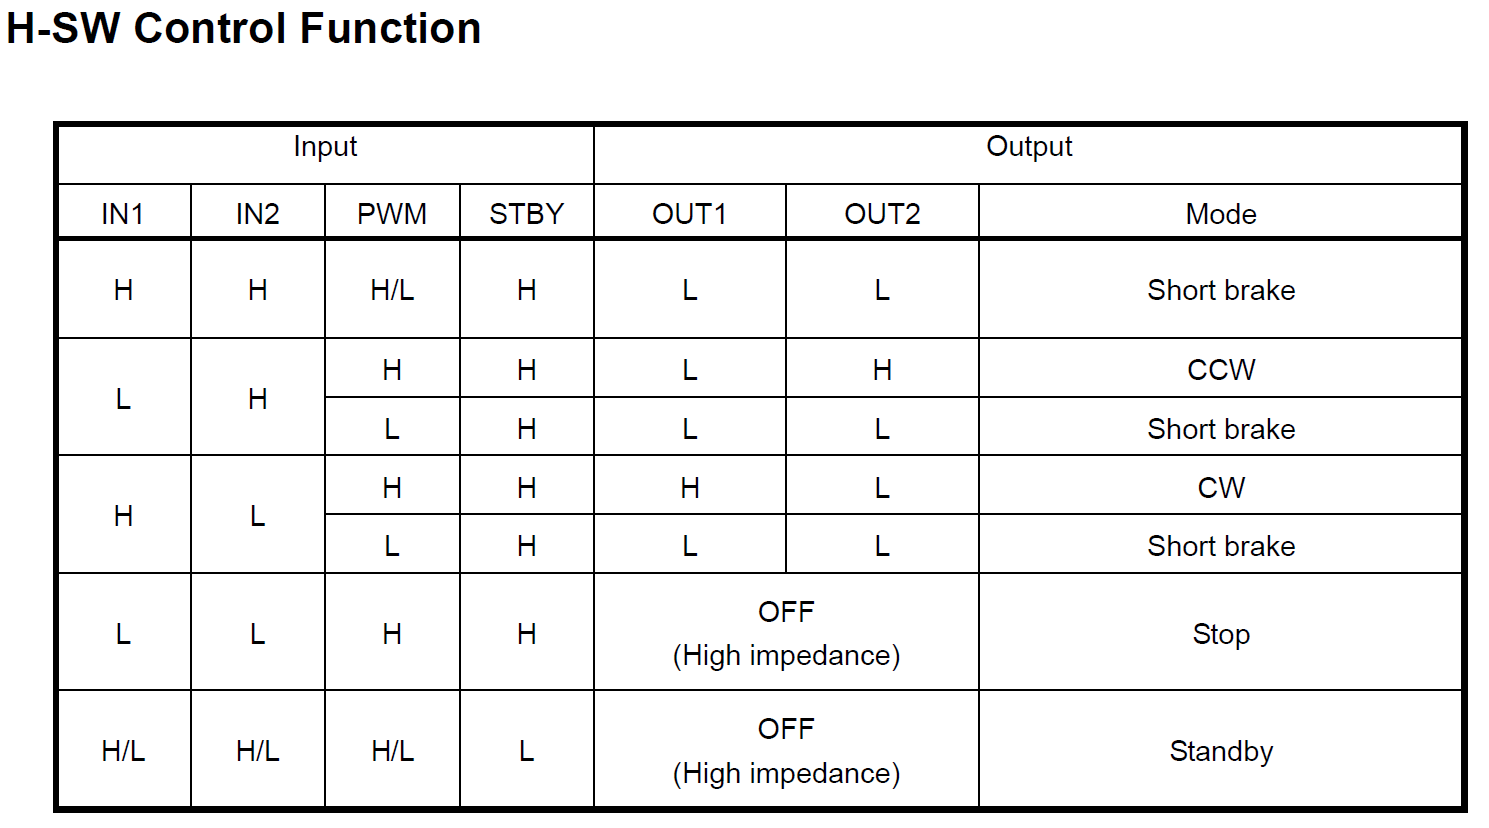
\includegraphics[width=12cm]{photos/prelim/motorcontrol.PNG}
    \caption{The Toshiba TB6612FNG's control code.}
\end{figure}

This chip features 4 signal to control each output to each motor. The inputs include a standby signal to enable and disable to chip, 2 input signals to dictate the operating mode such as counter-clockwise (CCW) or clockwise (CW) turning direction, and the PWM signal to indicate when to spin (H, signal high) and when to "short brake" (L, signal low). A high signal occurs when a voltage is applied at the input, as dictated by the datasheet where low occurs when it is connected to a low voltage such as ground. Instead of simply stopping supplying current when the PWM signal goes low, the chip slightly brakes the motor due to the fact it was just spinning and has momentum making it want to keep spinning. The operating mode, off, would however disconnect the motor from power. This chip also sources power to be supplied to the motors from a source thats capable of supplying more current than the microcontrollers output. Thus, the speed, direction, and behavior of a DC motor can be controlled by a microcontroller when utilizing this type of chip.

\end{document}